% !TeX root=../main.tex
\chapter{روش پژوهش و چهارچوب پیشنهادی}
%\thispagestyle{empty}

\section{مقدمه}

در فصل پیشین، مبانی نظری ناوبری ربات‌های متحرک و رویکردهای مبتنی بر یادگیری تقویتی عمیق مورد بررسی قرار گرفت و مزایا و محدودیت‌های چارچوب‌های موجود تحلیل شد. جمع‌بندی آن مباحث نشان داد که یادگیری تقویتی عمیق، به‌دلیل توانایی در یادگیری سیاست‌های تصمیم‌گیری از طریق تعامل با محیط، ظرفیت قابل توجهی برای ناوبری در محیط‌های دینامیکی و غیرقطعی دارد. با این حال، عملکرد موفق این رویکرد در یک کاربرد مهندسی، صرفاً به انتخاب یک الگوریتم یادگیری وابسته نیست؛ بلکه به نحوه فرمول‌بندی مسئله، تعریف مناسب فضای حالت و فضای کنش، طراحی تابع پاداش، لحاظ‌کردن قیود دینامیکی سامانه و انتخاب الگوریتم متناسب با ماهیت مسئله بستگی دارد.

بر این اساس، هدف این فصل تبیین روش‌شناسی پژوهش و ارائه چارچوب پیشنهادی برای ناوبری خودران اسکوتر چهارچرخ محرک در محیط‌های دینامیکی است. برای این منظور، ابتدا مفاهیم پایه و ضروری یادگیری تقویتی، شامل تعامل عامل و محیط، سیاست، تابع ارزش، تابع عمل-ارزش و اصل تصمیم‌گیری دنباله‌ای، در حد مورد نیاز برای فرمول‌بندی مسئله مرور می‌شوند. این مفاهیم زمینه لازم را برای بیان دقیق‌تر مسئله ناوبری اسکوتر در قالب یک مسئله یادگیری تقویتی فراهم می‌کنند.

در ادامه، مسئله ناوبری خودران اسکوتر به‌عنوان یک فرایند تصمیم‌گیری دنباله‌ای مدل‌سازی شده و اجزای اصلی آن شامل عامل، محیط، فضای حالت یا مشاهده، فضای کنش، تابع پاداش و شرایط پایان اپیزود تعریف می‌شوند. در این فرمول‌بندی، اسکوتر به‌عنوان عامل یادگیرنده در نظر گرفته می‌شود که در هر گام زمانی، بر اساس اطلاعات دریافتی از وضعیت خود، موقعیت نسبی هدف و وضعیت موانع محیط، فرمان حرکتی مناسب را انتخاب می‌کند. نتیجه این فرمان در محیط اعمال شده و بر اساس میزان پیشرفت به سمت هدف، حفظ ایمنی، اجتناب از برخورد و نرمی حرکت، پاداش یا جریمه به عامل اختصاص داده می‌شود.

با توجه به ماهیت پیوسته فضای کنش و دینامیکی بودن محیط، مسئله تعادل میان اکتشاف و بهره‌برداری نیز مورد توجه قرار می‌گیرد. در کاربرد حاضر، عامل باید علاوه بر یافتن مسیرهای مؤثر برای رسیدن به هدف، از رفتارهای پرخطر، نوسانی یا ناسازگار با قیود حرکتی اسکوتر اجتناب کند. از این رو، عواملی مانند اغتشاش حسگرها، رفتار پیش‌بینی‌ناپذیر موانع متحرک، محدودیت‌های سرعت و شتاب، و ضرورت تولید فرمان‌های نرم و قابل اجرا، به‌عنوان الزامات اصلی طراحی چارچوب یادگیری در نظر گرفته می‌شوند.

سپس خانواده‌های اصلی الگوریتم‌های یادگیری تقویتی، شامل روش‌های ارزش‌محور، روش‌های مبتنی بر گرادیان سیاست و چارچوب‌های کنشگر-منتقد، از نظر سازگاری با مسئله ناوبری اسکوتر مقایسه می‌شوند. این مقایسه با تمرکز بر معیارهایی مانند پایداری آموزش، کارایی نمونه، قابلیت کار با فضای کنش پیوسته، توانایی اکتشاف مؤثر و امکان تولید فرمان‌های کنترلی نرم انجام می‌شود. بر مبنای این تحلیل، الگوریتم مناسب برای هسته تصمیم‌گیری سامانه انتخاب شده و جایگاه آن در چارچوب پیشنهادی پژوهش مشخص می‌گردد.

در نهایت، این فصل با جمع‌بندی فرمول‌بندی مسئله و منطق انتخاب چارچوب الگوریتمی، مبنای لازم برای طراحی، پیاده‌سازی و ارزیابی سامانه ناوبری خودران در فصل‌های بعدی را فراهم می‌کند.

 
\section{تعریف، چارچوب تعامل و جایگاه یادگیری تقویتی در ناوبری}

یادگیری تقویتی به‌عنوان یکی از شاخه‌های اصلی یادگیری ماشین، چارچوبی برای یادگیری تصمیم‌گیری از طریق تعامل مستقیم عامل با محیط فراهم می‌کند. در این چارچوب، برخلاف یادگیری نظارتی که در آن خروجی مطلوب برای هر ورودی از پیش مشخص است، عامل یادگیرنده%
\LTRfootnote{Agent} %
با اجرای کنش%
\LTRfootnote{Action} %
در محیط%
\LTRfootnote{Environment} %
و دریافت بازخورد به‌صورت پاداش%
\LTRfootnote{Reward} %
، سیاست%
\LTRfootnote{Policy} %
تصمیم‌گیری خود را به‌تدریج بهبود می‌دهد. بنابراین، هدف یادگیری تقویتی صرفاً یادگیری یک نگاشت ایستا از ورودی به خروجی نیست، بلکه یادگیری یک راهبرد تصمیم‌گیری وابسته به وضعیت است که پیامدهای آینده تصمیم‌ها را نیز در نظر می‌گیرد. رابطه تعاملی میان عامل و محیط در چارچوب یادگیری تقویتی به‌صورت تصویری در شکل \ref{fig:RL_structure} نمایش داده شده است.
\begin{figure}[ht]
	\centering
	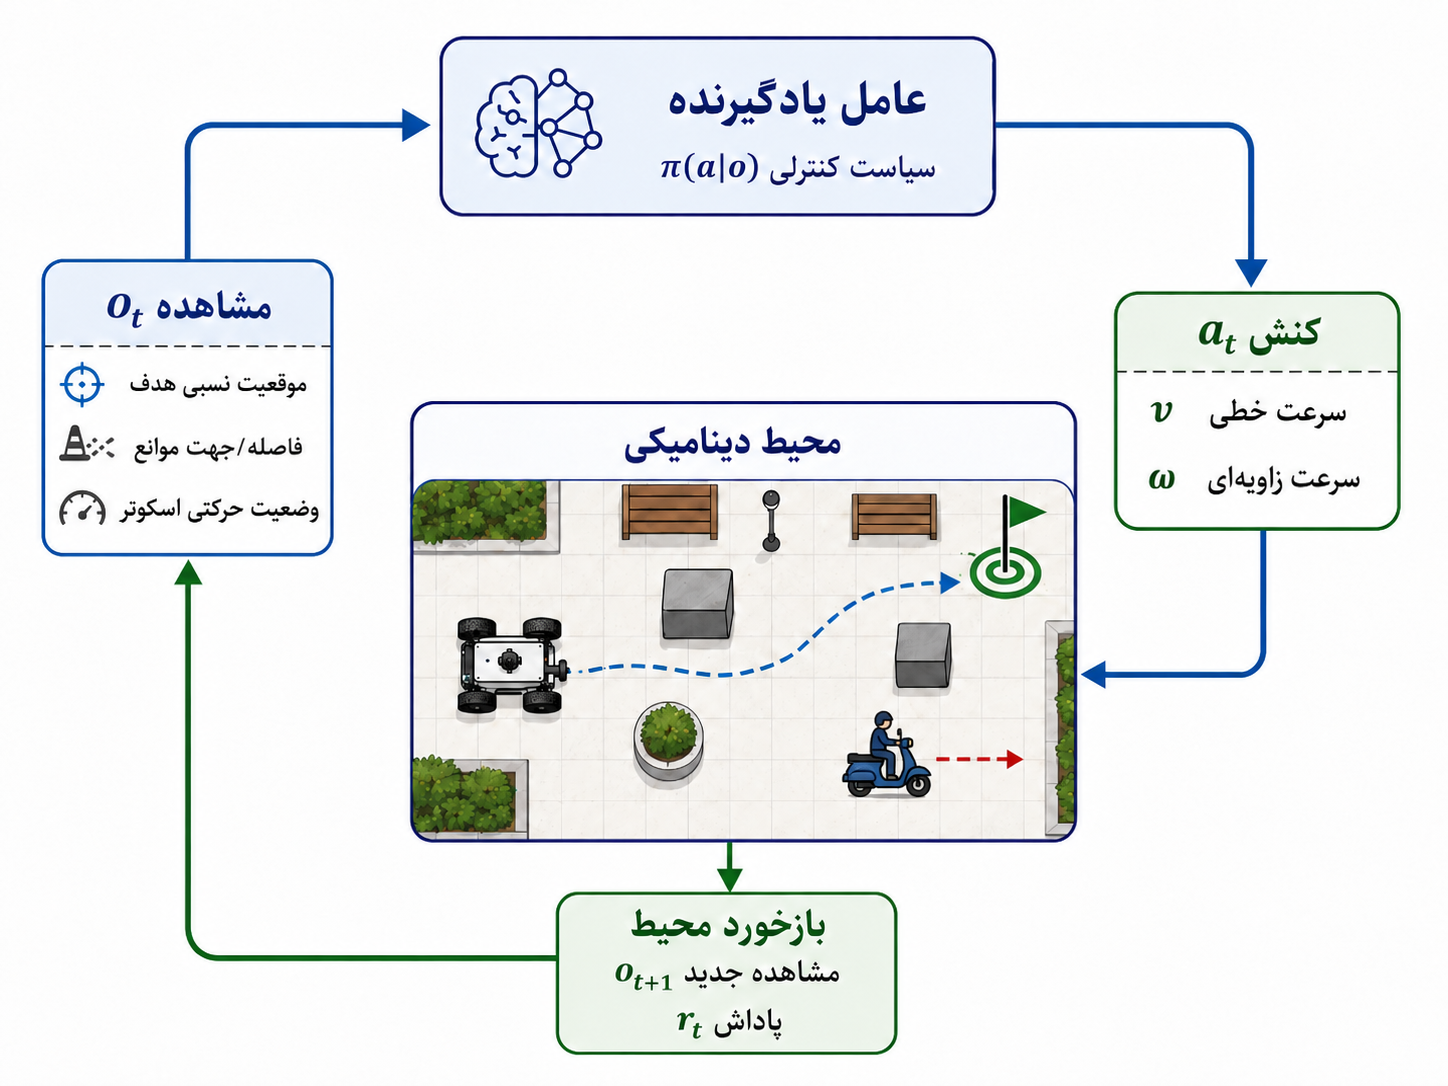
\includegraphics[width=0.85\textwidth]{img/RL_structure}
	\caption{چارچوب تعامل عامل و محیط در مسئله ناوبری خودران اسکوتر مبتنی بر یادگیری تقویتی}
	\label{fig:RL_structure}
\end{figure}

در ساده‌ترین توصیف، فرآیند یادگیری تقویتی به‌صورت یک چرخه تعاملی میان عامل و محیط بیان می‌شود. در هر گام زمانی ($t$)، عامل مشاهده فعلی خود از محیط را به‌صورت ($o_t$) دریافت می‌کند و بر اساس سیاست جاری، کنش ($a_t$) را انتخاب می‌نماید. سپس محیط در پاسخ به این کنش به وضعیت جدیدی منتقل شده و مقدار پاداش ($r_t$) را به عامل بازمی‌گرداند. این چرخه تا رسیدن به هدف، وقوع برخورد، اتمام زمان مجاز یا تحقق سایر شرایط پایان اپیزود ادامه می‌یابد. در حالت مشاهده‌پذیری کامل، مشاهده عامل می‌تواند معادل وضعیت محیط در نظر گرفته شود؛ اما در بسیاری از مسائل ناوبری، عامل تنها به بخشی از اطلاعات محیط دسترسی دارد و تصمیم‌گیری بر اساس مشاهده‌های محدود انجام می‌شود.

نکته اساسی در یادگیری تقویتی آن است که کیفیت یک کنش تنها بر اساس اثر لحظه‌ای آن ارزیابی نمی‌شود، بلکه تأثیر آن بر وضعیت‌های آینده نیز اهمیت دارد. از این رو، هدف عامل بیشینه‌سازی بازده تجمعی در طول زمان است. این ویژگی یادگیری تقویتی را برای مسائلی مانند ناوبری خودران مناسب می‌سازد؛ زیرا یک فرمان حرکتی در لحظه می‌تواند علاوه بر تغییر موقعیت فعلی، بر امکان اجتناب از موانع، حفظ فاصله ایمن، قابلیت توقف و انتخاب‌های بعدی سامانه نیز اثر بگذارد %
\cite{SuttonBarto2018}.

در مقایسه با یادگیری نظارتی، داده‌های آموزشی در یادگیری تقویتی به‌صورت مجموعه‌ای مستقل و برچسب‌خورده در اختیار عامل قرار نمی‌گیرند، بلکه در اثر تعامل عامل با محیط تولید می‌شوند. بنابراین، توزیع داده‌های تجربه‌شده به سیاست رفتاری عامل وابسته است. این ویژگی باعث می‌شود فرآیند یادگیری در یادگیری تقویتی ماهیتی پویا و وابسته به تصمیم‌های قبلی عامل داشته باشد. همچنین، در یادگیری تقویتی هدف به‌جای پیش‌بینی یک خروجی مشخص برای هر ورودی، بهینه‌سازی یک معیار کلی مانند مجموع پاداش‌های دریافتی در طول اپیزود است.

در مقایسه با یادگیری تقلیدی نیز، یادگیری تقویتی الزاماً به وجود نمونه‌های رفتاری از یک عامل خبره وابسته نیست. این موضوع در مسائل ناوبری اهمیت دارد؛ زیرا تهیه مسیرها یا فرمان‌های مرجع برای تمام شرایط ممکن محیط، به‌ویژه در حضور موانع متحرک و سناریوهای پیش‌بینی‌ناپذیر، دشوار و گاهی غیرعملی است. در مقابل، یادگیری تقویتی می‌تواند رفتار عامل را مستقیماً بر اساس اهدافی مانند رسیدن به مقصد، اجتناب از برخورد، کاهش زمان حرکت و تولید فرمان‌های نرم بهینه کند.

در مسئله ناوبری خودران اسکوتر چهارچرخ محرک، تصمیم‌گیری پیوسته و وابسته به شرایط محیطی به‌صورت طبیعی وجود دارد. انتخاب فرمان حرکتی در هر لحظه، نه‌تنها وضعیت فعلی اسکوتر را تغییر می‌دهد، بلکه نحوه مواجهه آن با موانع، امکان حفظ ایمنی و قابلیت ادامه مسیر در گام‌های بعدی را نیز تحت تأثیر قرار می‌دهد %
\cite{Zhu2021}. %
 
 از این رو، چارچوب یادگیری تقویتی به دلیل ماهیت تعاملی، هدف‌محور و مناسب برای تصمیم‌گیری دنباله‌ای، گزینه‌ای قابل توجیه برای مدل‌سازی و حل مسئله ناوبری در این پژوهش محسوب می‌شود. در ادامه، این مسئله در قالب فرایند تصمیم‌گیری مارکوف فرمول‌بندی شده و اجزای اصلی آن برای سامانه ناوبری اسکوتر تعریف می‌شوند.%


\section{فرایند تصمیم‌گیری مارکوف و فرمول‌بندی ریاضی مسئله}

برای مدل‌سازی رسمی مسئله ناوبری خودران در چارچوب یادگیری تقویتی، از مفهوم فرایند تصمیم‌گیری مارکوف%
\LTRfootnote{Markov Decision Process -- MDP} %
استفاده می‌شود. این چارچوب یک مدل ریاضی برای توصیف مسائل تصمیم‌گیری دنباله‌ای است که در آن، در حالت ایده‌آل، فرض می‌شود وضعیت فعلی شامل تمام اطلاعات لازم برای تصمیم‌گیری بوده و اثر تاریخچه گذشته به‌صورت ضمنی در آن نهفته است %
\cite{SuttonBarto2018}. در مسائل عملی مانند ناوبری رباتی، این فرض معمولاً به‌صورت تقریبی برقرار بوده و سیستم در عمل ماهیت مشاهده‌ناقص دارد که می‌تواند در قالب تعمیم‌یافته POMDP
 نیز تفسیر شود.

یک MDP به‌صورت یک پنج‌تایی تعریف می‌شود:

\begin{equation}\label{eq:MDP}
	\mathcal{M} = (\mathcal{S}, \mathcal{A}, \mathcal{P}, \mathcal{R}, \gamma)
\end{equation}

که در آن:

\begin{itemize}
	\item $\mathcal{S}$: فضای حالت شامل نمایش فشرده‌ای از وضعیت سیستم است
	\item $\mathcal{A}$: مجموعه کنش‌های قابل انتخاب توسط عامل است
	\item $\mathcal{P}(s_{t+1} \mid s_t, a_t)$: تابع انتقال یا دینامیک محیط است
	\item $\mathcal{R}(s_t, a_t)$: تابع پاداش برای ارزیابی کیفیت تصمیم‌ها است
	\item $\gamma \in [0,1]$: ضریب کاهشی پاداش‌های آینده است
\end{itemize}

در این چارچوب، هدف عامل یادگیرنده یافتن سیاستی ($\pi(a \mid s)$) است که امید ریاضی بازده تجمعی کاهش یافته را بیشینه کند:

\begin{equation}\label{eq:cumulative_reward}
	J(\pi) = \mathbb{E}_\pi \left[ \sum_{t=0}^{\infty} \gamma^t r_t \right]
\end{equation}

که در آن $r_t$ پاداش دریافتی در گام زمانی $t$ است.

\subsubsection*{کاربرد MDP در مسئله ناوبری اسکوتر}

در مسئله ناوبری خودران اسکوتر چهارچرخ محرک، اجزای MDP به‌صورت زیر تعریف می‌شوند:

\begin{itemize}
	\item \textbf{حالت ($\mathcal{S}$):} برداری از متغیرهای پیوسته شامل موقعیت نسبی و فاصله تا هدف، وضعیت حرکتی اسکوتر (سرعت خطی و زاویه‌ای) و اطلاعات استخراج‌شده از حسگرهای محیطی و موانع میباشد. این نمایش به‌گونه‌ای طراحی شده است که وابستگی به مختصات مطلق کاهش یافته و قابلیت تعمیم‌پذیری سیاست افزایش یابد
	
	\item \textbf{کنش ($\mathcal{A}$):} فرمان‌های حرکتی پیوسته شامل سرعت خطی و سرعت زاویه‌ای اسکوتر
	
	\item \textbf{تابع انتقال ($\mathcal{P}$):} دینامیک حرکتی اسکوتر و تغییرات محیط که به‌صورت صریح مدل‌سازی نشده و از طریق تعامل عامل با محیط شبیه‌سازی‌شده به‌صورت ضمنی نمونه‌برداری می‌شود
	
	\item \textbf{تابع پاداش ($\mathcal{R}$):} تابعی ترکیبی و وزن‌دار از مؤلفه‌های مختلف شامل پیشرفت به سمت هدف، فاصله از موانع، جریمه برخورد، و میزان نرمی حرکات کنترلی
	
	\item \textbf{ضریب کاهشی ($\gamma$):} پارامتری که اهمیت پاداش‌های آینده را نسبت به پاداش‌های لحظه‌ای تنظیم می‌کند
\end{itemize}

در نتیجه، مسئله ناوبری به‌صورت یک مسئله بهینه‌سازی سیاست در نظر گرفته می‌شود که در آن عامل باید سیاستی بیاموزد که در بلندمدت منجر به حرکت ایمن، پایدار و کارا در محیط‌های دینامیکی شود. با توجه به محدودیت دسترسی کامل به وضعیت محیط و وجود اغتشاش در مشاهدات، این چارچوب در عمل می‌تواند به‌صورت یک POMDP نیز تفسیر گردد.

\section{خاصیت مارکوف و ملاحظات مشاهده ناقص در ناوبری واقعی}

در تعریف کلاسیک فرایند تصمیم‌گیری مارکوف، فرض می‌شود که وضعیت $s_t$ به‌گونه‌ای تعریف شده است که تمامی اطلاعات لازم برای پیش‌بینی آینده را در خود دارد؛ به‌طوری‌که انتقال به وضعیت بعدی تنها به $(s_t, a_t)$ وابسته بوده و به تاریخچه کامل گذشته وابستگی مستقیم ندارد. این ویژگی به‌عنوان خاصیت مارکوف شناخته می‌شود\cite{SuttonBarto2018}.

به‌صورت رسمی، این خاصیت به شکل زیر بیان می‌شود:

\begin{equation}\label{markov_assumption}
	P(s_{t+1} \mid s_t, a_t, s_{t-1}, a_{t-1}, \dots) 
	=
	P(s_{t+1} \mid s_t, a_t)
\end{equation}

در مسائل مهندسی و به‌ویژه کاربردهای رباتیکی، این فرض معمولاً به‌صورت کامل برقرار نیست. در ناوبری خودران اسکوتر، محدودیت‌های حسگری، اغتشاش اندازه‌گیری و عدم دسترسی به وضعیت کامل محیط باعث می‌شود عامل به‌جای وضعیت واقعی $s_t$ تنها یک مشاهده $o_t$ از محیط دریافت کند.

این شرایط منجر به مدل‌سازی مسئله در قالب POMDP می‌شود، در حالی که عامل تنها به اطلاعات ناقص و فیلترشده از وضعیت واقعی دسترسی دارد.

\subsection*{تحلیل مسئله ناوبری اسکوتر از منظر POMDP}

در مسئله ناوبری خودران، عوامل متعددی موجب مشاهده ناقص می‌شوند، از جمله:

\begin{itemize}
	\item پوشش محدود حسگرها و عدم مشاهده کامل محیط اطراف
	\item عدم قطعیت در رفتار موانع متحرک و هدف
	\item وجود اغتشاش در اندازه‌گیری موقعیت و سرعت
	\item عدم دسترسی مستقیم به برخی متغیرهای محیطی مانند سرعت واقعی موانع
\end{itemize}

بنابراین، از دیدگاه نظری، این مسئله به‌طور دقیق‌تر در قالب POMDP قابل توصیف است. با این حال، در عمل در بسیاری از روش‌های یادگیری تقویتی، از جمله روش‌های مبتنی بر شبکه‌های عصبی، این مسئله با توسعه فضای حالت به یک تقریب MDP تبدیل می‌شود.

در این راستا، بردار حالت معمولاً با افزودن اطلاعات تکمیلی مانند چند گام اخیر مشاهدات، سرعت فعلی سیستم و تخمین وضعیت موانع غنی‌سازی می‌شود تا تا حد امکان خاصیت مارکوف به‌صورت تقریبی برقرار گردد. در این پژوهش نیز، مسئله ناوبری اسکوتر در قالب یک MDP تقریبی مدل‌سازی شده است؛ به‌گونه‌ای که فضای حالت با ترکیب اطلاعات حرکتی و سنسوری طراحی شده تا وابستگی به تاریخچه کاهش یافته و امکان استفاده از الگوریتم‌های استاندارد یادگیری تقویتی مانند روش‌های کنشگر-منتقد فراهم گردد.

\section{سیاست، تابع ارزش و هدف بهینه‌سازی در یادگیری تقویتی}

پس از فرمول‌بندی مسئله ناوبری در قالب \lr{MDP}، لازم است معیارهای ارزیابی تصمیم‌گیری و ساختار بهینه‌سازی سیاست مشخص شوند. در یادگیری تقویتی، هدف اصلی یافتن سیاستی $\pi$ است که بازده تجمعی مورد انتظار را بیشینه کند \cite{SuttonBarto2018}.

سیاست $\pi$ بیان‌کننده قاعده تصمیم‌گیری عامل برای انتخاب کنش در هر وضعیت است و می‌تواند به‌صورت احتمالی یا قطعی تعریف شود. در حالت کلی، سیاست تصادفی به‌صورت زیر نمایش داده می‌شود:

\begin{equation}\label{probable_policy}
	\pi(a \mid s) = P(a_t = a \mid s_t = s)
\end{equation}

در مسائل با فضای عمل پیوسته مانند ناوبری رباتی، سیاست معمولاً به‌صورت تابع پارامتری (نظیر شبکه عصبی) مدل‌سازی می‌شود و خروجی آن مستقیماً کنش کنترلی سیستم است.

هدف عامل در این چارچوب، بیشینه‌سازی بازده تعریف‌شده به‌صورت مجموع کاهش یافته پاداش‌ها است:

\begin{equation}\label{return}
	G_t = \sum_{k=0}^{\infty} \gamma^k r_{t+k}
\end{equation}

در این رابطه، ضریب $\gamma$ میزان اهمیت پاداش‌های آینده را نسبت به پاداش‌های آنی تنظیم می‌کند و نقش مهمی در تعادل میان رفتار واکنشی و تصمیم‌گیری بلندمدت در ناوبری دارد.

برای ارزیابی کیفیت سیاست، از توابع ارزش استفاده می‌شود. تابع ارزش حالت و تابع ارزش کنش به‌ترتیب به‌صورت زیر تعریف می‌شوند:

\begin{equation}\label{state_value_function}
	V^\pi(s) = \mathbb{E}_\pi [G_t \mid s_t = s]
\end{equation}

\begin{equation}\label{action_value_function}
	Q^\pi(s,a) = \mathbb{E}_\pi [G_t \mid s_t = s, a_t = a]
\end{equation}

در این روابط، تابع $Q$ نشان می‌دهد که انتخاب یک کنش مشخص در یک وضعیت معین چه تأثیری بر بازده بلندمدت سیستم خواهد داشت؛ موضوعی که در مسائل کنترلی مانند ناوبری خودران اهمیت مستقیم دارد.

ساختار بازگشتی این توابع از رابطه بلمن
\LTRfootnote{Bellman}
 تبعیت می‌کند:

\begin{equation}\label{bellman_equation}
	V^\pi(s) = 
	\mathbb{E}_{a \sim \pi, s' \sim \mathcal{P}}
	\left[
	r(s,a) + \gamma V^\pi(s')
	\right]
\end{equation}

در عمل، این رابطه مبنای محاسباتی بسیاری از الگوریتم‌های یادگیری تقویتی مبتنی بر تخمین ارزش و به‌روزرسانی تدریجی سیاست است.

در مسئله ناوبری خودران اسکوتر، تابع ارزش بیانگر کیفیت یک وضعیت از نظر ترکیبی از معیارهایی مانند فاصله تا هدف، میزان نزدیکی به موانع و امکان ادامه مسیر ایمن است. به‌طور مشابه، تابع $Q$ اثر انتخاب یک فرمان حرکتی خاص را بر آینده سیستم ارزیابی می‌کند.

بر این اساس، هدف نهایی یادگیری به‌صورت مسئله بهینه‌سازی سیاست تعریف می‌شود:

\begin{equation}
	\pi^* = \arg\max_\pi \;
	\mathbb{E}_\pi \left[ \sum_{t=0}^{\infty} \gamma^t r_t \right]
\end{equation}

این فرم‌بندی، پایه نظری استفاده از روش‌های یادگیری تقویتی در طراحی سیاست کنترلی ناوبری اسکوتر را فراهم می‌کند.
\section{اکتشاف و بهره‌برداری و نقش آن در محیط‌های دینامیکی}

یکی از چالش‌های مهم در یادگیری تقویتی، ایجاد تعادل میان اکتشاف%
\LTRfootnote{Exploration} %
و بهره‌برداری%
\LTRfootnote{Exploitation} %
است. در این میان، بهره‌برداری به استفاده از دانش فعلی عامل برای انتخاب بهترین کنش شناخته‌شده اشاره دارد، در حالی‌که اکتشاف به معنای آزمون کنش‌های جدید برای بهبود سیاست در بلندمدت است \cite{SuttonBarto2018}.

در محیط‌های دینامیکی، این تعادل اهمیت بیشتری پیدا می‌کند، زیرا انتخاب‌های اشتباه در فاز اکتشاف می‌تواند مستقیماً منجر به رفتارهای ناایمن یا غیرقابل پیش‌بینی در سیستم‌های کنترلی مانند ناوبری رباتی شود.

\subsection{اهمیت اکتشاف در ناوبری دینامیکی}

در مسئله ناوبری خودران اسکوتر، اکتشاف با محدودیت‌های عملی و ایمنی همراه است. حضور موانع متحرک، اغتشاش حسگرها و حساسیت بالای سیستم به فرمان‌های کنترلی باعث می‌شود که رفتارهای تصادفی شدید یا بدون قید، منجر به برخورد یا ناپایداری حرکتی شوند. از این رو، طراحی سازوکار اکتشاف باید به‌گونه‌ای باشد که ضمن حفظ امکان یادگیری، از تولید کنش‌های پرریسک جلوگیری کند.

\subsection{روش‌های رایج برای مدیریت اکتشاف}

در فضای عمل پیوسته، روش‌های متداول مدیریت اکتشاف شامل افزودن اغتشاش به سیاست و یا مدل‌سازی احتمالی سیاست هستند. در روش‌هایی مانند ،DDPG سیاست به‌صورت قطعی تعریف شده و برای ایجاد اکتشاف، اغتشاش تصادفی به خروجی اضافه می‌شود:

\begin{equation}
	a_t = \mu_\theta(s_t) + \mathcal{N}_t
\end{equation}

این روش امکان اکتشاف موضعی را فراهم می‌کند، اما تنظیم شدت اغتشاش در سیستم‌های کنترلی حساس مانند ناوبری اسکوتر می‌تواند چالش‌برانگیز باشد؛ زیرا اغتشاش زیاد موجب رفتارهای ناپایدار و اغتشاش کم منجر به گیر افتادن در سیاست‌های زیرینه می‌شود.

در مقابل، در روش‌های مبتنی بر سیاست تصادفی، خروجی به‌صورت یک توزیع احتمالی مدل‌سازی می‌شود:

\begin{equation}
	\pi_\theta(a \mid s) = \mathcal{N}(\mu_\theta(s), \sigma_\theta(s)^2)
\end{equation}

در این حالت، میزان اکتشاف به‌صورت درونی در ساختار سیاست کنترل می‌شود.

رویکرد پیشرفته‌تر در این زمینه، بیشینه‌سازی آنتروپی سیاست است که در آن عامل علاوه بر بیشینه‌سازی پاداش، به حفظ تنوع در تصمیم‌گیری نیز تشویق می‌شود:

\begin{equation}
	J(\pi) =
	\mathbb{E}_\pi
	\left[
	\sum_{t=0}^{\infty}
	\gamma^t
	\left(
	r_t + \alpha \mathcal{H}(\pi(\cdot \mid s_t))
	\right)
	\right]
\end{equation}

این رویکرد امکان کنترل تدریجی تعادل میان اکتشاف و بهره‌برداری را فراهم می‌کند و از نظر پایداری یادگیری در محیط‌های دینامیکی عملکرد مناسبی دارد \cite{Haarnoja2018SAC}.

\subsection{تحلیل در مسئله ناوبری اسکوتر}

در مسئله ناوبری خودران، اکتشاف نامناسب می‌تواند منجر به رفتارهای پرریسک مانند برخورد با موانع، انحراف شدید از مسیر یا نوسان در فرمان‌های حرکتی شود. از این رو، روش‌هایی که اکتشاف را به‌صورت کنترل‌شده و نرم در سیاست ادغام می‌کنند، نسبت به روش‌های مبتنی بر اغتشاش خام مناسب‌تر هستند.

در همین راستا، روش‌های مبتنی بر بیشینه‌سازی آنتروپی، به‌ویژه در قالب الگوریتم‌های کنشگر-منتقد نرم، گزینه مناسبی برای این مسئله محسوب می‌شوند؛ زیرا امکان ایجاد تعادل پایدار میان یادگیری، اکتشاف و ایمنی را فراهم می‌کنند.
\section{مقایسه الگوریتم‌های یادگیری تقویتی برای ناوبری خودران}

پس از تبیین چارچوب یادگیری تقویتی و ویژگی‌های مسئله ناوبری، انتخاب الگوریتم مناسب نقش کلیدی در عملکرد نهایی سامانه دارد. این انتخاب باید بر اساس ویژگی‌های فضای عمل پیوسته، دینامیک محیط و الزامات ایمنی صورت گیرد.

\subsection{روش‌های مبتنی بر مقدار}

روش‌هایی مانند Q-learning و DQN بر تقریب تابع ارزش کنش $Q(s,a)$ متکی هستند. این روش‌ها اساساً برای فضای عمل گسسته طراحی شده‌اند و استفاده از آن‌ها در مسائل پیوسته نیازمند گسسته‌سازی فضای عمل است. در مسئله ناوبری اسکوتر، گسسته‌سازی فضای کنش (سرعت خطی و زاویه‌ای) منجر به کاهش دقت کنترل و تولید حرکات ناپیوسته می‌شود. بنابراین این دسته از روش‌ها برای این کاربرد مناسب نیستند.

\subsection{روش‌های مبتنی بر گرادیان سیاست}

در این روش‌ها، سیاست به‌صورت مستقیم پارامتردهی شده و با استفاده از گرادیان تابع هدف بهینه می‌شود:

\begin{equation}
	\nabla_\theta J(\theta) =
	\mathbb{E}
	\left[
	\nabla_\theta \log \pi_\theta(a|s)\, Q^\pi(s,a)
	\right]
\end{equation}

الگوریتم‌هایی مانند Reinforce از این چارچوب استفاده می‌کنند، اما در مسائل پیچیده به‌دلیل واریانس بالا و ناپایداری یادگیری، عملکرد محدودی دارند.

\subsection{الگوریتم PPO}

PPO یکی از روش‌های پایدارتر در خانواده گرادیان سیاست است که با محدود کردن تغییرات سیاست در هر به‌روزرسانی، پایداری آموزش را افزایش می‌دهد\cite{Schulman2017PPO}. با این حال PPO، یک روش on-policy است و نیازمند جمع‌آوری داده جدید در هر به‌روزرسانی می‌باشد. این ویژگی در مسائل رباتیکی با هزینه نمونه‌برداری بالا، مانند ناوبری واقعی، محدودکننده است.

\subsection{روش DDPG}

DDPG یک الگوریتم off-policy برای فضای عمل پیوسته است که از سیاست قطعی و اغتشاش اکتشافی برای یادگیری استفاده می‌کند\cite{Lillicrap2016}. این روش اگرچه برای کنترل پیوسته مناسب است، اما حساسیت بالایی به تنظیم هایپرپارامترها دارد و در محیط‌های دینامیکی ممکن است ناپایداری در یادگیری و رفتارهای غیرهموار ایجاد شود.

\subsection{روش‌های مبتنی بر بیشینه‌سازی آنتروپی}

در چارچوب بیشینه‌سازی آنتروپی، سیاست علاوه بر بیشینه‌سازی پاداش، به حفظ تنوع در تصمیم‌گیری نیز تشویق می‌شود. الگوریتم SAC بر این اصل استوار است\cite{Haarnoja2018SAC}.

مزایای اصلی این روش عبارت‌اند از:
\begin{itemize}
	\item کارایی نمونه بالا به دلیل off-policy بودن
	\item پایداری بیشتر نسبت به DDPG
	\item تعادل خودکار میان اکتشاف و بهره‌برداری
	\item مناسب برای فضای عمل پیوسته
\end{itemize}

\subsection{جمع‌بندی و انتخاب الگوریتم}

با توجه به ویژگی‌های مسئله ناوبری اسکوتر شامل فضای عمل پیوسته، محیط دینامیکی، وجود اغتشاش و حساسیت بالا به ایمنی، الگوریتمی مورد نیاز است که هم پایدار باشد و هم کارایی نمونه بالایی داشته باشد.

در میان روش‌های بررسی‌شده، الگوریتم‌های مبتنی بر بیشینه‌سازی آنتروپی و به‌ویژه SAC بیشترین انطباق را با نیازهای این مسئله دارند. این الگوریتم امکان یادگیری پایدار، اکتشاف کنترل‌شده و عملکرد مناسب در فضای پیوسته را فراهم می‌کند، و بنابراین به‌عنوان هسته روش پیشنهادی این پژوهش انتخاب شده است.